\documentclass[11pt]{article}
\usepackage[a4paper,margin=1in]{geometry}
\usepackage{amsmath,amssymb,amsthm,mathtools}
\usepackage{hyperref}
\usepackage{needspace}
\usepackage{graphicx}
\usepackage[section]{placeins}

\title{Perfect Closure and Zeta Zeros: The Critical Line as a Square-Root Mirror}
\author{John Van Geem / RQM Technologies}
\date{April 2026}

\newtheorem{proposition}{Proposition}

\begin{document}
\maketitle

\begin{abstract}
This entry paper defines Perfect Closure in the zeta setting and isolates the key local theorem: for each prime route, the critical line $\operatorname{Re}(s)=1/2$ is the unique amplitude-balance line. The point is not to claim that a local prime equation proves global zero placement. The point is to state, with explicit algebra, why the half-line is the only place where conjugate amplitudes line up in magnitude for each prime route.

We use
\[
p^{-s}=p^{-\sigma}e^{-it\log p}
\]
for $s=\sigma+it$, and define the local imbalance
\[
B_p(\sigma)=\left|p^{-\sigma}-p^{-(1-\sigma)}\right|.
\]
Writing $\sigma=1/2+\delta$ gives
\[
B_p(1/2+\delta)=2p^{-1/2}|\sinh(\delta\log p)|,
\]
so $B_p(\sigma)=0$ if and only if $\sigma=1/2$. We then define
\[
\Xi(t)=\xi\!\left(\frac12+it\right),\qquad C(t)=|\Xi(t)|^2,
\]
and use $\Xi(t_n)=0$ as the complex closure condition referenced by later papers. No proof of RH is claimed.
\end{abstract}

\Needspace{10\baselineskip}
\section*{Reader Guide}
This paper answers one question: \textbf{what is the complex spectral trace?}
Paper 1 is intentionally narrow. It prepares language and algebra that later papers reuse, and it does so without claiming more than the equations establish.

When this paper says ``complex spectral trace,'' it means a value $t_n$ such that
\[
\Xi(t_n)=0,
\]
where $\Xi(t)=\xi(1/2+it)$ is the completed residual on the critical line. The sections below build the local-amplitude story first, then define this global residual condition.

\Needspace{10\baselineskip}
\section{Perfect Closure in the zeta setting}
A \textbf{Perfect Closure event} is the vanishing of a chosen closure residual built from zeta data.

\begin{itemize}
  \item Local residual: prime-route imbalance $B_p$.
  \item Global residual: completed critical-line magnitude $C(t)=|\Xi(t)|^2$.
\end{itemize}

The local residual tells us where amplitude symmetry is possible route-by-route. The global residual tells us where the completed object reaches zero. Keeping these levels separate helps avoid over-claiming: local balance is structural support, while zero formation is global analytic behavior.

\Needspace{10\baselineskip}
\section{Prime route and square-root balance}
For prime $p>1$ and $s=\sigma+it$,
\[
p^{-s}=p^{-\sigma}e^{-it\log p}.
\]
This factorization splits each route into:
\begin{enumerate}
  \item an amplitude part, $p^{-\sigma}$, controlled by the real coordinate $\sigma$, and
  \item a phase part, $e^{-it\log p}$, controlled by the height variable $t$.
\end{enumerate}

On the critical line,
\[
p^{-(1/2+it)}=\frac1{\sqrt p}e^{-it\log p},
\]
and the conjugate route is
\[
p^{-(1/2-it)}=\frac1{\sqrt p}e^{+it\log p}.
\]
The key point is not that these two routes literally cancel one another term-by-term. The key point is that at $\sigma=1/2$ they carry equal amplitude $1/\sqrt p$ and opposite phase direction. This makes $\sigma=1/2$ the unique local balance line.

Another way to say the same thing: changing $t$ rotates phase, while changing $\sigma$ rescales amplitude. The critical line is where the conjugate pair has matched rescaling.

\begin{figure}[htbp]
  \centering
  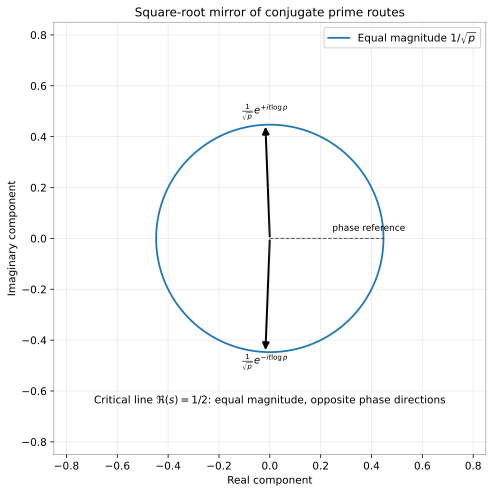
\includegraphics[width=0.78\textwidth]{../assets/figures/square-root-mirror-prime-routes.svg}
  \caption{The square-root mirror. On the critical line, the two conjugate prime routes have equal magnitude $1/\sqrt p$ and opposite phase direction, matching $p^{-(1/2\pm it)}=(1/\sqrt p)e^{\mp it\log p}$. This visualizes local amplitude balance and does not imply that an individual prime cancels $\zeta$.}
\end{figure}

\Needspace{10\baselineskip}
\section{Local imbalance theorem}
Define
\[
B_p(\sigma)=\left|p^{-\sigma}-p^{-(1-\sigma)}\right|.
\]
This residual compares two amplitudes reflected around $1/2$: one at $\sigma$, one at $1-\sigma$. If they are equal, local imbalance is zero.

Now write $\sigma=1/2+\delta$. Then
\[
\begin{aligned}
B_p\!\left(\frac12+\delta\right)
&=\left|p^{-1/2-\delta}-p^{-1/2+\delta}\right| \\
&=p^{-1/2}\left|p^{-\delta}-p^{\delta}\right| \\
&=p^{-1/2}\left|e^{-\delta\log p}-e^{\delta\log p}\right| \\
&=2p^{-1/2}|\sinh(\delta\log p)|.
\end{aligned}
\]
Each line has a simple role: factor out $p^{-1/2}$, rewrite powers as exponentials, then identify the hyperbolic sine form. The last line makes the zero condition transparent.

\begin{figure}[htbp]
  \centering
  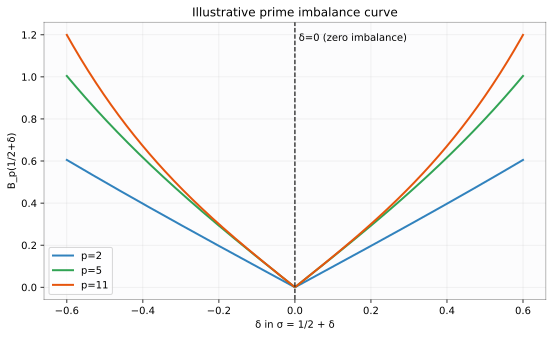
\includegraphics[width=0.80\textwidth]{../assets/figures/prime-imbalance-curve.svg}
  \caption{Illustrative imbalance curves for $B_p(1/2+\delta)=2p^{-1/2}|\sinh(\delta\log p)|$ at $p=2,5,11$, with $\delta=0$ marked as the zero-imbalance point. The chart supports Proposition 3.1 qualitatively and is not a numerical claim about zero locations.}
\end{figure}

\begin{proposition}
For every $p>1$,
\[
B_p(\sigma)=0 \iff \sigma=\frac12.
\]
\end{proposition}

\begin{proof}
Since $p^{-1/2}>0$,
\[
B_p(1/2+\delta)=0\iff \sinh(\delta\log p)=0.
\]
Because $\log p\neq0$ and $\sinh x=0\iff x=0$, we get $\delta=0$, i.e.\ $\sigma=1/2$. The converse is immediate.
\end{proof}

What this proposition gives is a clean local uniqueness statement. What it does not give is a global theorem about nontrivial zeros. It says where local amplitude mismatch vanishes, not where the full analytic continuation must vanish.

\Needspace{10\baselineskip}
\section{Optional finite-prime support}
For a finite set $p_1<\cdots<p_N$, define
\[
B_N(\sigma)^2=\sum_{j=1}^{N}B_{p_j}(\sigma)^2.
\]
Because each summand is nonnegative, $B_N(\sigma)=0$ if and only if every term is zero. By Proposition 3.1, that happens exactly at $\sigma=1/2$.

This finite statement is useful as an intuition check: aggregating finitely many local imbalances does not move the unique zero-imbalance line away from $1/2$.

\Needspace{10\baselineskip}
\section{Prime-power echo (brief context)}
In $\operatorname{Re}(s)>1$,
\[
\log\zeta(s)=\sum_p\sum_{k\ge1}\frac{p^{-ks}}{k}.
\]
In this bookkeeping language, $k=1$ terms are primary prime routes and $k\ge2$ terms are echo routes. The equation is included to remind the reader that the prime structure enters through layered harmonics, not through one isolated factor.

This section is context only. The local imbalance theorem does not rely on this expansion.

\Needspace{10\baselineskip}
\section{Completed residual and complex spectral trace}
Define
\[
\Xi(t)=\xi\!\left(\frac12+it\right),\qquad C(t)=|\Xi(t)|^2.
\]
The first equation chooses a completed residual on the critical line. The second turns it into a nonnegative scalar closure score. A closure event is then written as
\[
\Xi(t_n)=0.
\]
Equivalently, $C(t_n)=0$. This is the exact complex spectral trace condition that Papers 2--5 carry forward.

The naming convention matters for readability in later papers:
\begin{itemize}
  \item ``trace'' refers to the observed complex-line condition $\Xi(t_n)=0$,
  \item ``eigenvalue'' refers to operator-side $t_n$ (Paper 4),
  \item ``mass-shell realization'' refers to physical norm mapping after scale conversion (Papers 4--5).
\end{itemize}

\Needspace{10\baselineskip}
\section{Non-claims and bridge}
\begin{itemize}
  \item No proof of RH.
  \item No claim of a zero-location algorithm.
  \item No claim that a single prime route cancels $\zeta$.
\end{itemize}

Bridge sentence: Paper 2 lifts the complex trace variable $1/2+it$ into quaternionic slice geometry $1/2+\mathbf u t$, so the same trace variable can be discussed across orientation slices.

\Needspace{10\baselineskip}
\section*{References}
\begin{enumerate}
  \item B. Riemann, \emph{Ueber die Anzahl der Primzahlen unter einer gegebenen Groesse} (1859).
  \item E. C. Titchmarsh and D. R. Heath-Brown, \emph{The Theory of the Riemann Zeta-Function}, 2nd ed., Oxford Univ. Press, 1986.
  \item H. M. Edwards, \emph{Riemann's Zeta Function}, Dover, 2001.
\end{enumerate}

\end{document}
